\chapter{Optymalizacja metodą roju cząstek - Particle Swarm Optimizaton}
\section*{Wprowadzenie}
Znalezienie najlepszej możliwej konfiguracji elementów konstrukcyjnych, zapewniającej poprawnie przeniesienie obciążeń statycznych, zapewniającej komfort dynamiczny i najlepiej możliwie taniej jest zadaniem, które na co dzień towarzyszy projektantom mostów. Takie zadanie może kojarzyć się intuicyjnie z pojęciem optymalizacji, czyli wyborem najlepszego z wielu rozwiązań, pozwalającego osiągnąć cel lub cele. \cite{Szymczak1995} określa następuje elementy, jakie powinno zawierać poprawnie sformułowane zadanie optymalizacji
\begin{itemize}[noitemsep]
	\item kryteria optymalizacji - miarę spełnienia danego celu,
	\item parametry optymalizacji - parametry systemu, które są stałe lub niezależne od projektanta, 
	\item zmienne projektowe - parametrów systemu zależne od projektanta,
	\item ograniczenia - elementy określające zakres dopuszczalnych rozwiązań. 
\end{itemize}
Kryterium optymalizacji powinno w sposób wymierny pozwolić na ocenę danego rozwiązania. Podstawowymi kryteriami stosowanymi w przypadku konstrukcji może być koszt jej wykonania, ilość materiału czy nakład pracy. Kryterium, które decyduje o wyborze najlepszego rozwiązania nazywane jest funkcją celu. W przypadku wielu kryteriów, jednym z rozwiązań upraszających proces optymalizacji jest stworzenie jednej funkcji celu, łączącej wszystkie kryteria z zastosowaniem wag dla poszczególnych elementów. Odbywa się to zazwyczaj na zasadzie kombinacji liniowej:
\begin{equation}
	F=\sum_{i=1}^{n}w_i F_i
\end{equation}
gdzie $w_i$ to współczynnik określający wagę kryterium $F_i$. W pracy został zastosowane rozwiązanie optymalizacji wielokryterialnej. W takim przypadku optymalizacja polega na minimalizowaniu lub maksymalizowaniu jednocześnie kilku funkcji celu. Zagadnienie zostanie omówione teoretycznie w punkcie \ref{sect: multiobjective_opt}. 

W przypadku konstrukcji, parametry projektowe to założone wartości opisujące ustrój, które nie ulegają zmianie w procesie optymalizacji.  Mogą być one narzucone przez względy technologiczne bądź normowe \parencite{Szymczak1995}, lub wynikać z innych założeń projektowych. Z kolei zmienne projektowe $x_i$, jak sama nazwa wskazuje, mogą się zmieniać w procesie optymalizacji i zależą od projektanta. Wybór konkretnych $m$ zmiennych projektowych tworzy rozwiązanie w postaci wektora $\vect{x}=[x_1,x_2,\dots,x_m]^T$, będącego punktem w przestrzeni $m$-wymiarowej.

Z reguły wartości zmiennych projektowych muszą spełniać szereg obostrzeń. Wynikają one ponownie ze względów technologicznych, normowych lub innych uznanych za istotne przez projektanta. Z tego powodu, na zmienne projektowe $\vect{x}$ narzucone są ograniczenia. Wektor, który spełnia wszystkie ograniczenia nazywany jest dopuszczalnym. W analizie konstrukcji budowlanych ograniczeniami mogą być wymogi wytrzymałościowe, eksploatacyjne - zarówno statyczne jak i dynamiczne - czy też warunki stateczności. \textbf{DODAĆ OPIS MATEMATYCZNY OGRANICZEŃ}


\section{Klasyfikacja problemów i metod optymalizacji}
Wszystkie powyższe elementy definiują problem optymalizacji. Każdy z nich może przyjmować różne postaci co będzie miało znaczący wpływ przede wszystkim na wybór metody rozwiązania problemu. \cite{Tesch2016} zaproponował następującą klasyfikację problemów optymalizacji zależnie od elementów charakterystycznych je definiujących:
\begin{itemize}[noitemsep]
	\item Liczba funkcji celu
	\begin{itemize}[noitemsep]
		\item pojedyncza funkcja celu,
		\item wiele funkcji celu.
	\end{itemize}
	\item Liczba ekstremów lokalnych
	\begin{itemize}[noitemsep]
		\item funkcja unimodalna - funkcja jest ciągła i posiada jedno ekstremum w rozpatrywanym przedziale,
		\item funkcja multimodalna - problem posiada więcej niż jedno ektremum lokalne w rozpatrywanym zakresie,
	\end{itemize}
	\item Liniowość funkcji celu
	\begin{itemize}[noitemsep]
		\item problem programowania liniowego - funkcja celu i ograniczenia są liniowe,
		\item problem programowania nieliniowego - funkcja celu lub ograniczenia nie są liniowe,
	\end{itemize}
	\item Rodzaj zmiennych projektowych
	\begin{itemize}[noitemsep]
		\item ciągłe - zmienne projektowe są liczbami rzeczywistymi w zadanym przedziale,
		\item dyskretne - zmienne projektowe są liczbami całkowitymi w zadanym przedziale,
		\item mieszane - w problemie występują zarówno zmienne ciągłych jak i dyskretnych ,
	\end{itemize}
\end{itemize}

Klasyfikacje zawarte w klasycznych pozycjach dotyczących optymalizacji podają również ogólny podział ze względu na to czy zmienne projektowe są liczbami czy funkcjami \parencite{Szymczak1995,Findeisen1980}.

Rodzaj problemu optymalizacji ogranicza wybór metody, którą można użyć do jego rozwiązania. W literaturze algorytmy tradycyjne dzielone są ze względu na sposób przeszukiwania na: analityczne, enumeratywne oraz losowe \parencite{Goldberg1995}. W skrócie, pierwsze opierają się na stworzeniu i rozwiązaniu układu równań, powstałego przez przyrównanie gradientu funkcji celu do zera. Metody te wymagają obliczenia pochodnych funkcji i mają charakter lokalny, szukając optymalnego rozwiązania wokół punktu, a nie w całym dopuszczalnym obszarze. W realnych przypadkach są to trudne do zaakceptowania warunki i metody te mają raczej ograniczony zakres zastosowań. Metody enumeracyjne polegają na obliczaniu funkcji celu dla kolejnych rozwiązań dopuszczalnych. W literaturze przedmiotu inną spotykaną nazwą tej metody jest "systematyczne przeszukiwanie". Pomimo naturalności metody i jej prostoty jest to najmniej efektywna klasa metod, co jest jej główną wadą. Działanie metod losowych jest podobne do systematycznego przeszukiwania, z tą różnicą że kolejne rozwiązania są dobierane w sposób losowy, a nie uporządkowany. Metody losowe w ogólności nie pozwalają efektywniej uzyskać optymalnego rozwiązania niż enumeratywne. Przedstawione konwencjonalne metody są albo wysoce wyspecjalizowne i swoim zastosowaniem obejmują wąskie spektrum problemów, albo są mało efektywne w szerokim zakresie zastosowań. 

Znając ograniczenia metod tradycyjnych, poszukiwano innych, które dzięki wykorzystaniu maszyn cyfrowych mogą stać się jednocześnie znacznie bardziej efektywne niż metody enumeratywne oraz jednocześnie pozwalają na rozwiązanie znacznie bardziej różnorodnych zadań niż metody analityczne. W odpowiedzi powstały algorytmy, które doboru coraz lepszego rozwiązania dokonują wykorzystując randomizację, ale nie są w zupełności losowe. Są to tak zwane algorytmy heurystyczne i w rozwiniętej wersji metaheurystyczne. Wykorzystują one doświadczenie powstałe na bazie przeprowadzonych prób i uczą się na ich podstawie szukając coraz lepszego wyniku, wykorzystując przy tym mechanizm randomizacji. Są to algorytmy zapewniające dobre rozwiązanie przy poświęceniu rozsądnej ilości czasu. Ponadto, większość algorytmów metaheurystycznych ma charakter globalny i nie ogranicza się do funkcji unimodalnych. Niemniej jednak, pomimo niewątpliwych zalet, należy pamiętać że algorytmy metaheurystyczne są z natury przybliżone. W związku z tym nie gwarantują, że optymalny wynik zostanie w ogóle odnaleziony. Najbardziej popularne algorytmy metaheurystyczne są inspirowane zachowaniami zaobserwowanymi w naturze \parencite{FisterJr.2013}. Główne mechanizmy ich działania mogą być zaczerpnięte z praw fizyki (np. Algorytm Przeszukiwania Grawitacyjnego \parencite{Rashedi2009}), biologii (np. Algorytmy Genetyczne \parencite{Goldberg1995}) czy inteligencji stadnej (np. Optymizacja Rojem Cząstek \parencite{Kennedy1995,Eberhart2001}).
Podsumowując i odwołując się do wyżej przytoczonej klasyfikacji problemów optymalizacji, algorytmy ich rozwiązania \cite{Tesch2016} podzielił według następujących kryteriów:
\begin{itemize}[noitemsep]
	\item Różniczkowalność funkcji celu
	\begin{itemize}[noitemsep]
		\item Wymagające pochodnej - algorytmy tej kategorii wymagają istnienia dwukrotnej pochodnej funkcji celu.
		\item Niewymagające pochodnej - algorytmy tej klasy nie wymagają ciągłości funkcji celu oraz jej pochodnej.
	\end{itemize}
	\item Liczba jednocześnie rozważanych rozwiązań
	\begin{itemize}[noitemsep]
		\item Jednopunktowe - w jednej chwili rozważane jest jedno rozwiązanie. W kolejnych krokach algorytmu jest ono modyfikowane w celu uzyskania lepszego rozwiązania.
		\item Wielopunktowe - jednocześnie odbywa się analiza wielu rozwiązań, które mają wpływ na wynik końcowy.
	\end{itemize}
	\item Mechanizmy losowości
	\begin{itemize}[noitemsep]
		\item Deterministyczne - rozwiązania są wyznaczane jedynie na podstawie danych wejściowych i wyznaczonych parametrów.
		\item Stochastyczne - zmienne projektowe są wybierane z uwzględnieniem czynnika losowego.
		\item Hybrydowe - algorytm zawiera oba mechanizmy wyboru kolejnego rozwiązania.
	\end{itemize}
\end{itemize}

\section{Określenie funkcji celu i wybór metody optymalizacji}
Wpływ poszczególnych rozwiązań konstrukcyjnych obiektu na jego odpowiedź dynamiczną zalicza się do zagadnień złożonych. 
Pierwszą funkcją celu postawionego problemu może być minimalizacja przyspieszeń pionowych pomostu w trakcie przejazdu. Jest to najbardziej najczęściej decydujący warunek eksploatacyjny mostu narzucony przez normę Europejską. Drugą pożądaną cechą może być poszukiwanie najtańszego obiektu (w uproszczeniu najmniejszej ilości materiału), przy spełnieniu wszystkich innych warunków wytrzymałościowych. Wybór metody optymalizacji, która została wykorzystana dokonano przez analizę rozpatrywanego zadania. Z uwagi na brak funkcyjnego opisu odpowiedzi dynamicznej modelu numerycznego zaniechano użycia metod analitycznych, wymagających obliczania pochodnych. Dodatkowo problem ma charakter globalny i nie wolno dopuścić do zakończenia poszukiwania w ekstremum lokalnym.  Odrzucono również metody losowe i systematycznego przeszukiwania z uwagi na długotrwałe wyznaczanie funkcji celu i bardzo nieefektywny algorytm. Kolejnym kryterium była uniwersalność algorytmu, ponieważ zaplanowano użycie go w dwóch zupełnie różnych problemach: kalibracji modelu i optymalizacji konstrukcji z punktu widzenia zachowania dynamicznego. Ostatnim kryterium była udokumentowana w literaturze skuteczność metody, w tym wykorzystanie jej w przypadkach analizy i oceny konstrukcji. Powyższe warunki spełniają metody metaheurystyczne. Spośród opisanych w literaturze wybrano metodę optymalizacji rojem cząstek.
\section{Opis algorytmu}
Optymalizacja rojem cząstek \teng{Particle Swarm Optimization (PSO)} jest metaheurystycznym, inspirowanym naturą algorytmem optymalizacji. W bazowej wersji powstał w roku 1995 \parencite{Kennedy1995a,Eberhart1995} i od tamtej pory ulegał wielu modyfikacjom, udoskonaleniom i rozszerzeniom. Metoda zakłada istnienie pewnej populacji - roju składającego się z $M$ cząstek. Każda cząstka o indeksie $i$ posiada trzy informacje $(\vect{x}_i,\vect{v}_i,\vect{p}_i)$. $\vect{x}_i$ i $\vect{p}_i$ są wektorami o długości $D$ oznaczającymi punkt w przeszukiwanej przestrzeni $\matr{X}$, gdzie $D$ jest liczbą zmiennych projektowych problemu. $\vect{x}_i$ oznacza aktualną pozycją cząstki w przestrzeni $\matr{X}$. Z kolei $\vect{p}_i$ określa najlepsze dotychczasowe położenie cząstki $i$ \teng{personal best (pbest)}. Jakość położenia określana jest przez wyznaczenie funkcji celu dla danej cząstki (np. zakładając minimalizację, mniejsza wartość funkcji celu jest lepsza od większej). Jeżeli funkcja celu dla nowego położenia cząstki jest lepsza niż zachowana w pamięci (pbest) to wektor $\vect{p}_i$ jest aktualizowany do nowej wartości. $\vect{v}_i$ jest również wektorem o długości $D$ i oznacza różnicę pomiędzy nowym położeniem w chwili $t+1$ i poprzedzającym w chwili $t$:
\begin{equation} \label{eq: pso_position}
	\vect{x}_i^{t+1}=\vect{x}_i^t+\vect{v}_i^{t+1}
\end{equation}
 Jako że wektor $\vect{v}_i$ decyduje o kolejnym położeniu cząstki nazywany jest również wektorem prędkości. Współrzędne wektora $\vect{v}_i$ z kroku $t$ uaktualniane są w kolejnej iteracji $t+1$ w następujący sposób:
\begin{equation} \label{eq: pso_velocity}
	\vect{v}_{i}^{t+1}=\theta\vect{v}_i^t+\alpha\vect{u}_1^t\circ (\vect{n}_i^t-\vect{x}_i^t)+\beta\vect{u}_2^t\circ(\vect{p}_i^t-\vect{x}_i^t)
\end{equation}
gdzie wektory $\vect{u}_1^t$ i $\vect{u}_2^t$ zawierają zestawy losowych liczb o rozkładzie jednostajnym z zakresu [0,1], ustalonych w chwili czasowej $t$. Symbol $(\circ)$ oznacza iloczyn skalarny. Parametry $\alpha$, $\beta$ i $\theta$ w pierwotnej wersji algorytmu są stałymi. W zależności od zastosowanej topologii roju, $\vect{n}_i$ oznacza najlepsze rozwiązanie $\vect{p}_i$ spośród dostępnych sąsiadów. W jednej z najpopularniejszych i najbardziej intuicyjnych wersji stosowana jest topologia gbest, w której $\vect{n}_i$ przyjmuje najlepszą wartość $\vect{p}_i$ spośród wszystkich cząstek.
\subsubsection{Parametry algorytmu PSO}
Każdy składnik prędkości spełnia określoną rolę. Pierwszy jest związany z bezwładnością i utrzymuje on bieżącą trajektorię cząstki. Parametr $\theta$ w ogólności zmniejsza prędkość, zapewniając lepszą zbieżność rozwiązania \parencite{Blackwell2019}. Jego wartość może być stała lub zmienna w trakcie analizy. Współczynniki $\alpha$ i $\beta$ odpowiadają za przyspieszenie na bazie odpowiednio własnych i społecznych doświadczeń. 
\cite{Clerc2002} wyznaczyli wartości $\theta=0.7968$, $\alpha=1.4962$ i $\beta=1.4962$ jako optymalne z punktu widzenia działania algorytmu. Przyjęcie równości $\alpha=\beta$ oznacza, że na prędkość cząstki równy wpływ mają doświadczenia własne i sąsiadów. Do podobnych rezultatów doszli \cite{Shi1998}. \cite{Xu2007} podaje przykład zmiennego wariantu, gdzie $\theta$ zmniejsza swoją wartość liniowo od 0.9 do 0.4, a parametry $\alpha$ i $\beta$ są stałe i równe 2.0. \cite{Poli2007} obszernie opisali metody wyznaczania wartości parametrów algorytmu.
\subsubsection{Topologie roju}
Topologa roju odpowiada za zachowanie społeczne cząstek roju.  Określa ona sąsiedztwo, z którym cząstka może się komunikować i wymieniać doświadczeniem. Definiuje również liderów, za którymi podążać będą pozostałe cząstki. Topologie dzielą się na dwie główne grupy: globalne \teng{global best (gbest))} i lokalne \teng{local best (lbest)}. Schemat topologii można przedstawić za pomocą grafów, w których węzły oznaczają cząstki, a krawędzie możliwość komunikacji z inną cząstką. Trzy najczęściej występujące w literaturze przedmiotu topologie to:
\begin{itemize}
	\item topologia pierścieniowa (Rys. \ref{fig: pso_topologies1}),
	\item topologia pełnego grafu (Rys. \ref{fig: pso_topologies2}),
	\item topologia von Neumanna (Rys. \ref{fig: pso_topologies3}).
\end{itemize}
\begin{figure}[h]
	\centering
	\subfloat[Topologia pierścieniowa]{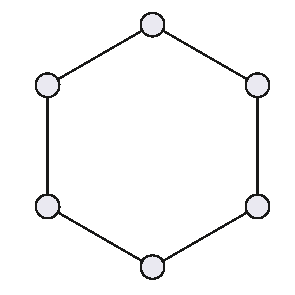
\includegraphics[width=0.3\linewidth]{/PSO/topology/pierscien.pdf} \label{fig: pso_topologies1}}
	\subfloat[Topologia pełnego grafu]{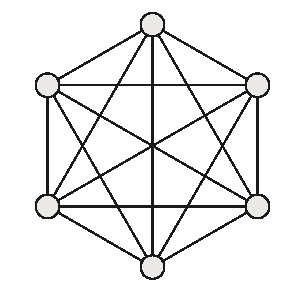
\includegraphics[width=0.3\linewidth]{/PSO/topology/global.pdf} \label{fig: pso_topologies2}}
	\subfloat[Topologia von Neumanna]{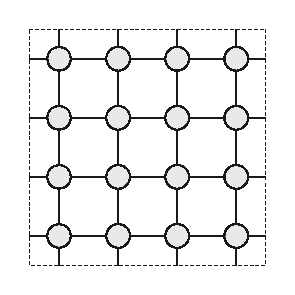
\includegraphics[width=0.3\linewidth]{/PSO/topology/neumann.pdf} \label{fig: pso_topologies3}}
	\captionsetup{justification=centering}
	\caption{Schematy wybranych topologi komunikacji pomiędzy cząstkami w metodzie optymalizacji rojem cząstek}
	\label{fig: pso_topologies}
\end{figure}
Przyjęta topologia roju ma istotny wpływ na zachowanie i efektywność algorytmu. Topologie należące do rodziny gbest osiągają szybciej zbieżność, ale istnieje większe ryzyko na utknięcie w minimum lokalnym gdy funkcja celu nie jest unimodalna. Innymi słowy przynosi ona precyzyjniejsze rozwiązanie, ale mniej dokładnie przeszukuje obszar. Przy wykorzystaniu rodziny lbest efekt jest odwrotny. Ograniczona jest komunikacja jedynie do wąskiego grona sąsiadów, przez co algorytm zbiega do rozwiązania wolniej. Zwiększa to szansę na dokładniejsze przeszukanie obszaru, ale zmniejsza precyzję ostatecznego wyniku. Topologie mogą być również podzielone na statyczne i dynamiczne. Pierwsze utrzymują swoją strukturę przez cały czas wykonywania algorytmu, drugie zmieniają swoje właściwości wraz z postępem obliczeń. Najczęściej topologiach dynamicznych populacja rozpoczyna od małej liczby sąsiadów żeby w trakcie wykonywania algorytmu ich liczba stopniowo wzrastała \parencite{Poli2007}. Warto podkreślić, że w klasycznej wersji algorytmu położenie cząstki w przestrzeni $\matr{X}$ nie ma wpływu na początkowy wybór sąsiedztwa zgodnie z założoną topologią.

Jedyną topologią z rodziny gbest jest topologia pełnego grafu (Rys. \ref{fig: pso_topologies2}). Każda cząstka może przekazywać informację o najlepszym położeniu ze wszystkimi innymi. W tym wariancie wektor $\vect{n}_i$ w formule (\ref{eq: pso_velocity}) jest równy dla wszystkich cząstek i odpowiada najlepszemu dotychczasowemu położeniu całej populacji. Z kolei pierwszą i najprostszą topologią lbest jest topologia pierścieniowa (Rys. \ref{fig: pso_topologies1}). Komunikacja jest zapewnione jedynie pomiędzy najbliższymi sąsiadami: cząstka o indeksie $i$ wymienia informację o najlepszym położeniu jedynie z cząstkami o indeksach $i-1$ i $i+1$. Trzecia wymieniona topologia von Neumanna należy również do rodziny lbest, ale reprezentuje kompromis pomiędzy przypadkami skrajnymi: topologią pierścieniową i pełnego grafu (Rys. \ref{fig: pso_topologies3}). Pozwala ona na wymianę informacji z czterema sąsiadami.\parencite{Kennedy2002} wykonali szereg testów obliczeniowych dla zróżnicowanych problemów dla wielu topologii. W tym teście topologia von Neumanna otrzymała najwyższą sumaryczną notę i jest opisana jako uniwersalna. Obszerne porównanie topologii wraz z historycznym opisem i powstania oraz efektywnością zostało zawarte w pracy \parencite{Blackwell2019}.

\subsection{Generacja populacji}
Początkowa populacja roju jest rozmieszczana w $D$-wymiarowej przestrzeni rozwiązań $\matr{X}$. Przyjęcie właściwej liczby cząstek nie jest kwestią ściśle określoną. \cite{Piotrowski2020} przeprowadzili obszerne studium dotyczące przyjęcia wstępnej liczebności populacji. Posłużyli się oni kilkudziesięcioma rzeczywistymi i testowymi problemami optymalizacji i ocenili 8 różnych wersji algorytmu. Na bazie analizy statystycznej stwierdzono, że klasycznie zalecane przyjęcie od 20 do 50 \parencite{Kennedy1995,Liang2006,Chen2012,Harrison2018} cząstek jest w przypadku wielu rzeczywistych problemów niewystarczające. Taka liczba sprawdza się jedynie w przypadku stosunkowo prostych problemów unimodalnych. Dla złożonych zagadnień i wersji algorytmu opisanej w niniejszej pracy autorzy podali poprawny zakres od 70 do 500 cząstek. Jednocześnie sformułowano również generalną wskazówkę, że dla wszystkich wariantów algorytmu bezpiecznym rozwiązaniem jest przyjęcie od 70 do 100 cząstek. Liczebność populacji w trakcie całej analizy jest zazwyczaj stała, chociaż istnieją modyfikacje algorytmu, które pozwalają na dodawanie cząstek w trakcie działania algorytmu.

\begin{figure}[h]
	\centering
	\subfloat[]{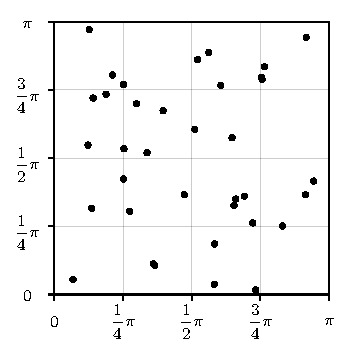
\includegraphics[width=0.35\linewidth]{/PSO/population/fig_population_random1.pdf} \label{fig: pso_gen_rand_1}}
	\subfloat[]{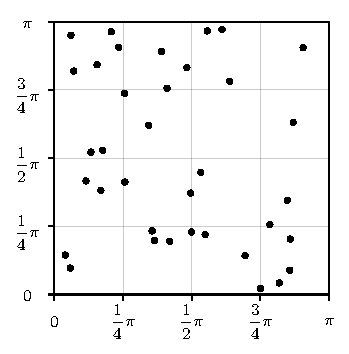
\includegraphics[width=0.35\linewidth]{/PSO/population/fig_population_random2.pdf} \label{fig: pso_gen_rand_2}}\\
	\subfloat[]{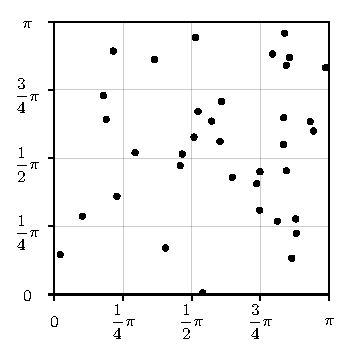
\includegraphics[width=0.35\linewidth]{/PSO/population/fig_population_random3.pdf} \label{fig: pso_gen_rand_3}}
	\subfloat[]{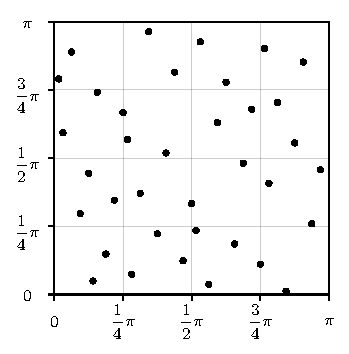
\includegraphics[width=0.35\linewidth]{/PSO/population/fig_population_halton.pdf}  \label{fig: pso_gen_halton}}
	\captionsetup{justification=centering}
	\caption{Przykłady rozkładu wygenerowanych populacji cząstek: (a)-(c) generacja losowa, (d) generacja z wykorzystaniem sekwencji Haltona}
	\label{fig: pso_gen_expl}
\end{figure}
Rozwiązania realnych zagadnień inżynierskich zazwyczaj cechują pewne ograniczenia, które przekładają się na dopuszczalny zakres zmiennych projektowych. Jeżeli wektor minimalnych wartości dopuszczalnych zmiennych projektowych zebrany zostanie w wektorze $x_{min}$, a maksymalnych jako $x_{max}$ to możliwe jest określenie hiperprostokąta o wierzchołkach $(x_{min},x_{max})$. Początkowe położenie cząstek odbywa się więc przez dobranie współrzędnych wektorów rozwiązań $x_i$, tak aby wszystkie cząstki znalazły się wewnątrz hiperprostokąta $(x_{min},x_{max})$. Pozycje początkowe mogą być wybierane przez użytkownika bądź losowane wewnątrz przestrzeni dopuszczalnych rozwiązań. Zakładając niewielką populację roju, istnieje spora szansa, że losowanie o jednorodnym rozkładzie nie zagwarantuje równomiernego pokrycia przestrzeni. Z tego powodu do generacji początkowej populacji niekiedy stosowane są deterministyczne algorytmy, które pozwalają uzyskać rozkład do złudzenia przypominający losowy, ale zapewniające jednocześnie równomierną dystrybucję w przestrzeni \parencite{Saliby2002}. Jedną z takich metod jest wykorzystanie sekwencji Haltona \parencite{Tesch2016}. Na rysunku \ref{fig: pso_gen_expl} pokazano przykłady rozkładu 36 początkowych cząstek w przestrzeni dwuwymiarowej. Trzykrotnie wylosowano populację za pomocą generatora pseudolosowego (\ref{fig: pso_gen_rand_1}$-$\ref{fig: pso_gen_rand_3}). Dla kontrastu przedstawiono punkty wygenerowane za pomocą sekwencji Haltona w takim samym zbiorze \ref{fig: pso_gen_halton}. W każdej z losowo wybranych populacji widoczne są obszary, które są gęsto pokryte i takie, w którym nie znajduje się żadna cząstka. Przy wykorzystaniu sekwencji Haltona przestrzeń jest pokryta znacznie bardziej równomiernie. Problem staje się tym bardziej istotny kiedy dotyczy małych populacji. Kiedy wyznaczenie funkcji celu jest bardzo kosztowne czasowo, a zadanie wielowymiarowe wykorzystanie sekwencji Haltona zwiększa pewność równomiernego rozkładu w całej przestrzeni.

%
\subsubsection{Warunki brzegowe}
Początkowa populacja roju jest losowana wewnątrz przestrzeni dopuszczalnych rozwiązań. Następnie wykorzystana jest inteligencja roju do przeszukania przestrzeni w celu znalezienia globalnego ekstremum. W trakcie kolejnych iteracji położenie cząstek zmieniane jest według wzorów (\ref{eq: pso_velocity}) i (\ref{eq: pso_position}). W trakcie obliczeń, w oryginalnej wersji algorytmu użytkownik nie ingeruje w proces przemieszczania się cząstek. Istnieje więc możliwość że wyznaczona prędkość wyprowadzi cząstkę poza obszar dopuszczalnych rozwiązań. Jest to szczególnie prawdopodobne kiedy ekstremum globalne znajduje się w pobliżu granicy rozwiązań dopuszczalnych \parencite{Xu2007}. Kiedy cząstka wyjdzie poza zakres dopuszczalnych rozwiązań jej wartość jest nieistotna (błędna) dla projektanta i nie powinna wpływać negatywnie na wynik końcowy. Jednym z rozwiązań jest obciążenie takiej cząstki karą. Do funkcji celu dodawana jest wartość, która drastycznie oddali wynik od najlepszego rezultatu (dla minimalizacji zwiększenie wyniku, a dla maksymalizacji pomniejszenie). 
Aby zniwelować efekt ucieczki z obszaru dopuszczalnego zastosowana może być prędkość maksymalna $V_{max}$, połączona ze współczynnikiem zaciskania \parencite{Eberhart2001a}. Zalecana prędkość maksymalna może być powiązana z rozpiętością zakresu zmiennych projektowych $V_{max}=X_{max}-X_{min}$. Drugim stosowanym zabiegiem jest zdefiniowanie warunków brzegowych. Modyfikują one parametry cząstki (położenie lub prędkość) jeżeli znajdzie się ona poza obszarem dopuszczalnych rozwiązań. W literaturze spotykane są cztery podstawowe rodzaje warunków brzegowych: absorbujący \teng{absorbing wall}, odbijający \teng{reflecting wall}, tłumiący \teng{damping wall} i niewidoczny \teng{invisible wall} \parencite{Robinson2004,Huang2005}. Efekt poszczególnych warunków brzegowych przy przekroczeniu przez cząstkę granicy danego wymiaru jest następujący:
\begin{itemize}[noitemsep]
	\item absorbujący - cząstka jest zatrzymywana na granicy, a składowa wektora prędkości w danym wymiarze jest zerowana,
	\item odbijający -  cząstka jest zatrzymywana na granicy, a znak składowej prędkości w danym wymiarze jest odwracany,
	\item tłumiący - cząstka jest zatrzymywana na granicy, a znak składowej prędkości w danym wymiarze jest odwracany i pomniejszany przez losowy mnożnik z zakresu $(0,1)$,
	\item niewidoczny - cząstka nie jest zatrzymywana na granicy, a wektor prędkości nie zmienia swojej definicji. Wartość funkcji celu nie jest wyznaczana.
\end{itemize} 
Na rysunku pokazano efekt oddziaływania na cząstkę każdego z warunków brzegowych w przestrzeni 2D o zmiennych projektowych d1 i d2. W swojej pracy, \parencite{Xu2007} zbadali dodatkowe warianty warunków opierające się powyższych założeniach, ale bez wymuszonej zmiany położenia cząstki, jedynie modyfikując prędkość. Autorzy podanych prac zgodnie określają warunek tłumiący jako najbardziej uniwersalny, a warunek niewidoczny jako najwydajniejszy w większości problemów.
\begin{figure}[h]
	\centering
	\subfloat[Absorbujący]{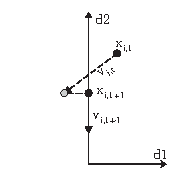
\includegraphics[width=0.25\linewidth]{/PSO/bounds/absorb.pdf} \label{fig: pso_bounds_abs}}
	\subfloat[Odbijający]{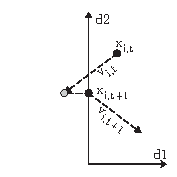
\includegraphics[width=0.25\linewidth]{/PSO/bounds/refl.pdf} \label{fig: pso_bounds_refl}}
	\subfloat[Tłumiący]{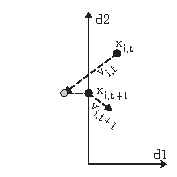
\includegraphics[width=0.25\linewidth]{/PSO/bounds/damp.pdf} \label{fig: pso_bounds_damp}}
	\subfloat[Niewidoczny]{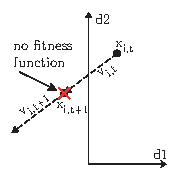
\includegraphics[width=0.25\linewidth]{/PSO/bounds/inv.pdf} \label{fig: pso_bounds_inv}}
	\captionsetup{justification=centering}
	\caption{Rodzaje warunków brzegowych wpływające na zachowanie cząstki wychodzącej poza zakres rozwiązań dopuszczalnych}
	\label{fig: pso_bounds_types}
\end{figure}
\subsubsection{Warunki zakończenia}
Algorytm PSO z każdą kolejną iteracją aktualizuje położenie cząstek i pamięć roju. Warunek zakończenia przeszukiwania przestrzeni może odbyć się w różny sposób. Najprostszą metodą jest określenie maksymalnej liczby aktualizacji roju, po której poszukiwanie zostanie zakończone. W tym przypadku na wstępie wiadomym jest ile iteracji zostanie wykonanych i przy znajomości czasu potrzebnego na oszacowanie funkcji celu możliwe jest określenie długości całego procesu optymalizacji. Podstawową wadą tego kryterium jest, że nie odnosi się w żaden sposób do jakości rozwiązania w ciągu trwania obliczeń. \parencite{Zielinski2007} przedstawili zestaw innych kryteriów, które uwzględniają zachowanie roju w trakcie poszukiwań. Wyróżniono następujące kryteria mogące wpływać na warunek zakończenie algorytmu:
\begin{itemize}[noitemsep]
	\item kryterium postępu - optymalizacja jest zatrzymana kiedy w określonej liczbie kolejnych iteracji nie nastąpi znaczące polepszenie ekstremum globalnego,
	\item kryterium ruchu - optymalizacja jest zatrzymywana kiedy położenie bieżącego ekstremum globalnego nie zmienia się istotnie w określonej liczbie kolejnych iteracji,
	\item kryterium dystrybucji populacji - optymalizacja jest zatrzymywana kiedy cząstki zgrupują się w jednym miejscu. Dystrybucja może być mierzona m. in. przez odchylenie standardowe położenia populacji, maksymalny dystans między cząstkami lub rozmiar roju mierzony przez długość boków hiperprostokąta, w którym w całości się mieści.  
	\item kryterium prędkości - optymalizacja jest zatrzymywana kiedy prędkość cząstek roju spadnie poniżej wartości minimalnej i nie wzrośnie przez określoną liczbę kolejnych iteracji. 
\end{itemize}
Wszystkie powyższe warunki mogą być łączone i użyte wedle potrzeb w zależności od specyfiki problemu optymalizacji. \cite{Banach2017} określił kryterium prędkości jako najbardziej uniwersalne, ponieważ nie dotyczy położenia cząstek roju i nie zależy od rozwiązywanego problemu optymalizacji. Uzasadnił, że nie wymaga ono znajomości wartości progowych najczęściej nieznanej funkcji celu oraz nie wymaga by wszystkie cząstki zbiegły w tym samym miejscu.

Podsumowując, algorytm podstawowej wersji metody optymalizacji rojem cząstek (PSO) przedstawiono na rysunku \ref{fig: pso_single_algorith}.
\begin{figure}[h]
	\centering
	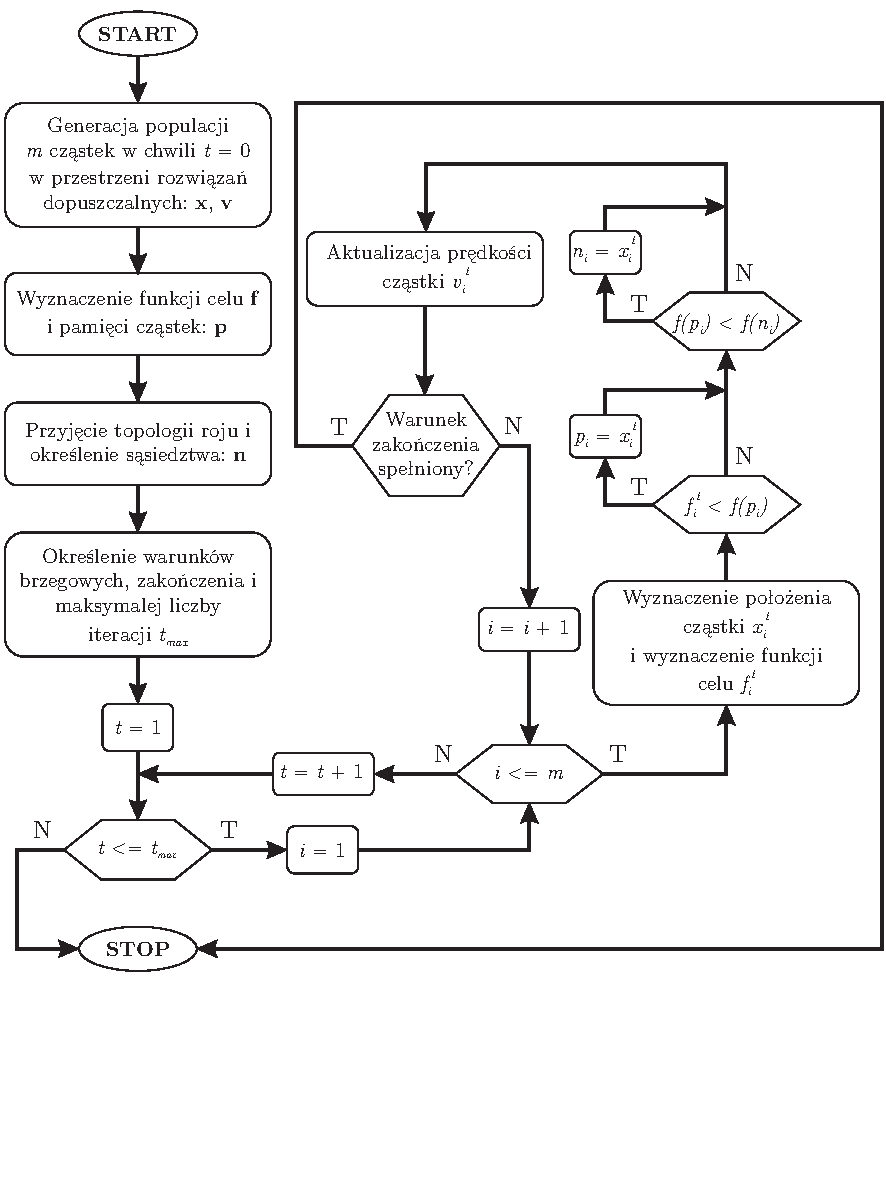
\includegraphics[trim= 0 100 0 0, clip, width=0.85\linewidth]{/PSO/algorithm/algorithm2.pdf} 
	\captionsetup{justification=centering}
	\caption{Podstawowy algorytm optymalizacji jednokryterialnej metodą roju cząstek PSO. Przypadek minimalizacji}
	\label{fig: pso_single_algorith}
\end{figure}


\subsection{Przykład teoretyczny}
W celu weryfikacji stosowanej metody przygotowano przykład teoretyczny. Zastosowano wariant minimalizacji funkcji celu za pomocą metody PSO. Zaimplementowano algorytm PSO w języku Python. Do testu wybrano funkcję multimodalną przedstawioną w pracy \parencite{Tesch2016} i daną wzorem:
\begin{equation} \label{eq: pso_test_func}
	f(x,y) = -5\sin{x}\sin{y}-5\sin{7x}\sin{7y}
\end{equation}
gdzie $x$, $y$ tworzą wektor zmiennych projektowych, a wartość funkcji $f(x,y)$ jest funkcją celu. Funkcję zwizualizowano w przestrzeni 3D na rysunku \ref{fig: pso_example_function}. Podobnie jak w pracy źródłowej przedział dopuszczalny dla każdej zmiennej projektowej to $[0,\pi]$. Wartość minimalna funkcji w tej dziedzinie jest znana i wynosi $f_{\text{min}}=-6$, dla punktu $(x,y)=(\frac{\pi}{2},\frac{\pi}{2})$.
\begin{figure}[h]
	\centering
	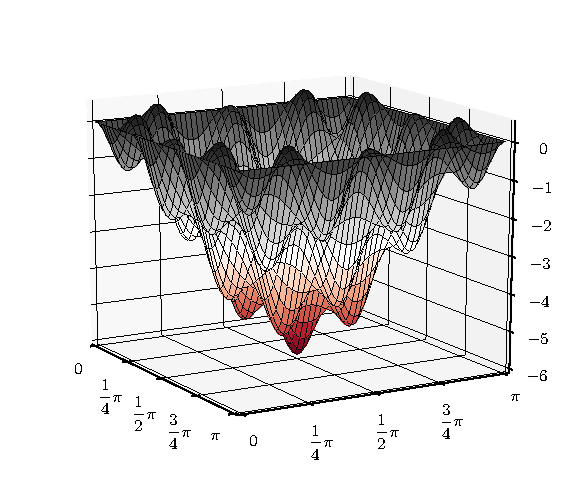
\includegraphics[trim= 0 0 0 10, clip,width=0.8\linewidth]{/PSO/testfunct/fig_3dplot_19_09_18.pdf} 
	\captionsetup{justification=centering}
	\caption{Wizualizacja funkcji testowej w przestrzeni trójwymiarowej}
	\label{fig: pso_example_function}
\end{figure}


Wygenerowano populację złożoną z 20 cząstek. Do generacji użyto wariant korzystający z sekwencji Haltona. Z uwagi na multimodalność funkcji celu zastosowano topologię z rodziny lbest - von Neumanna. Warunki brzegowe przyjęto typu niewidocznego. Parametry wektora prędkości (\ref{eq: pso_velocity}) ustawiono domyślnie równe: $\theta=0.7968$, $\alpha=1.4962$ oraz $\beta=1.4962$. Zatrzymanie algorytmu nastąpiło po wykonaniu założonej liczby aktualizacji całego roju równej 25. W konsekwencji całkowita liczba ewaluacji funkcji celu przez cząstki wynosi $25\cdot20=500$. Na rysunku \ref{fig: pso_convergence_plot} zaprezentowano diagram poprawy najlepszego rozwiązania znalezionego przez rój. Na rysunku \ref{fig: pso_test_func_all} pokazano 6 etapów z procesu poszukiwania przez rój minimum funkcji. Ostateczna znaleziona wartość minimum globalnego wynosi $f_{\text{min,25}}=-5.99$. Wartość ta została osiągnięta po około 400 ewaluacjach funkcji i jest bardzo bliska znanemu minimum globalnemu. Warto nadmienić, że już po 215 ewaluacjach odnaleziona zostało rozwiązanie o funkcji celu wynoszącej $f=-5.98$. Wizualizacja położenia cząstek roju w kolejnych iteracjach pokazuje, że wraz z postępem algorytmu, cząstki z rozproszonego układu skupiają się konsekwentnie wokół lidera. Topologia von Neumanna spowalnia ten proces. Opóźnia to znalezienie precyzyjnego rozwiązania, ale obszar dopuszczalny jest przeszukany dokładniej. Na kolejnych grafikach widać, że pomimo znalezienia punktu bliskiego teoretycznego minimum globalnego (Rys. \ref{fig: pso_test_func_2}) wciąż pozostają cząstki, które eksplorują pozostały obszar. Na podstawie powyższego testu uznano, że zaimplementowany algorytm PSO działa poprawnie.
\begin{figure}[h]
	\centering
	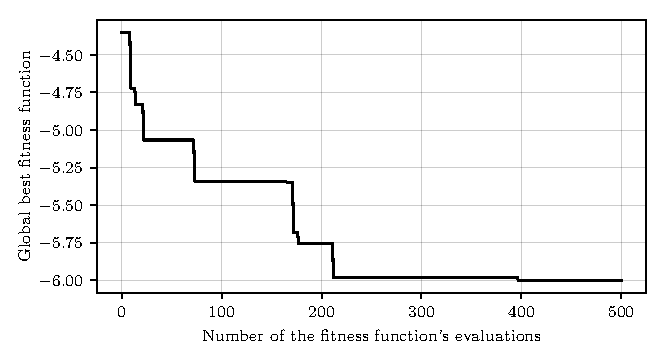
\includegraphics[trim=0 5 0 5, clip,width=0.75\linewidth]{/PSO/testfunct/fig_convergence11_30_59.pdf} 
	\captionsetup{justification=centering}
	\caption{Diagram postępu roju cząstek w poszukiwaniu minimum globalnego funkcji testowej}
	\label{fig: pso_convergence_plot} 
\end{figure}

\begin{figure}[H]
	\centering
	\subfloat[$f_{\text{min,0}}=-4.38$]{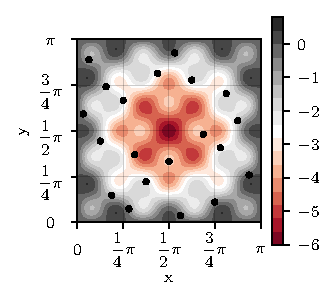
\includegraphics[trim=8 10 5 10, clip,width=0.33\linewidth]{/PSO/testfunct/fig_population_11_30_23.pdf} \label{fig: pso_test_func_1}}
	\subfloat[$f_{\text{min,5}}=-5.34$]{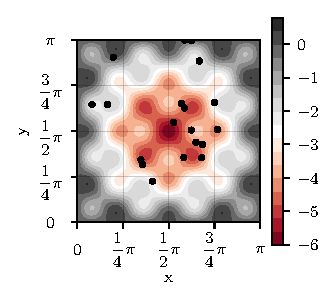
\includegraphics[trim=8 10 5 10, clip,width=0.33\linewidth]{/PSO/testfunct/fig_04_00.pdf} \label{fig: pso_test_func_2}}
	\subfloat[$f_{\text{min,10}}=-5.75$]{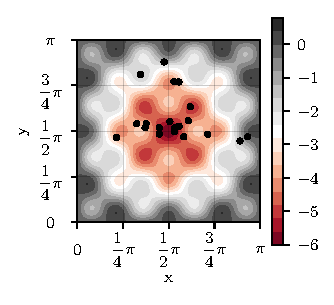
\includegraphics[trim=8 10 5 10, clip,width=0.33\linewidth]{/PSO/testfunct/fig_09_00.pdf} \label{fig: pso_test_func_3}}\\
	\subfloat[$f_{\text{min,15}}=-5.98$]{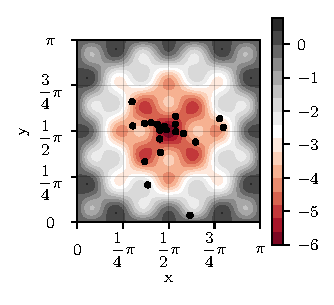
\includegraphics[trim=8 10 5 10, clip,width=0.33\linewidth]{/PSO/testfunct/fig_14_00.pdf} \label{fig: pso_test_func_4}}
	\subfloat[$f_{\text{min,20}}=-5.99$]{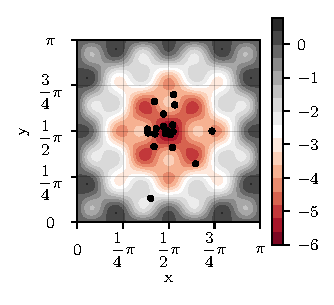
\includegraphics[trim=8 10 5 10, clip,width=0.33\linewidth]{/PSO/testfunct/fig_19_00.pdf} \label{fig: pso_test_func_5}}
	\subfloat[$f_{\text{min,25}}=-5.99$]{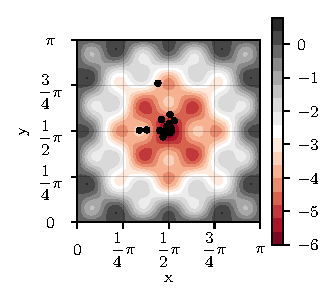
\includegraphics[trim=8 10 5 10, clip,width=0.33\linewidth]{/PSO/testfunct/fig_24_00.pdf} \label{fig: pso_test_func_6}}
	\captionsetup{justification=centering}
	\caption{Etapy rozwiązania testowego problemu optymalizacji dwuwymiarowej za pomocą roju cząstek. Minimum globalne znalezione przez rój oznaczono przez $f_{\text{min},t}$, gdzie indeks $t$ oznacza liczbę pełnych aktualizacji położenia roju. Za pomocą izomapy pokazano wartość funkcji celu na płaszczyźnie}
	\label{fig: pso_test_func_all}
\end{figure}



\section{Optymalizacja wielokryterialna} \label{sect: multiobjective_opt}
Jak wspomniano we wstępie rozdziału, rzeczywiste problemy inżynierskie rzadko sprowadzają się do jednego kryterium, którego optymalizacja dostarczy bezkompromisowo jedyne, idealne rozwiązanie. Najczęściej występuje kilka istotnych kryteriów stojących ze sobą w kontrze, które nie osiągają jednocześnie maksimum lub minimum dla tych samych wartości zmiennych projektowych. Jedna z metod radzenia sobie w takich przypadkach została już opisana i polega na liniowej kombinacji kryteriów, sprowadzając problem optymalizacji de facto do jednej funkcji celu. Wadą tego rozwiązania jest konieczność ustalenia skali ważności poszczególnych kryteriów jeszcze przed rozpoczęciem optymalizacji. Poza koniecznością ustalenia wag składników sumy, niekiedy trudno ustalić związki między zmiennymi projektowymi i sprowadzić wszystkie kryteria do jednego porównawczego, jakim jest na przykład koszt wykonania lub ilość materiału \parencite{Szymczak1995}. Inną metodą jest rozwiązanie problemu optymalizacji jako wielokryterialnego. Polega ona na jednoczesnej minimalizacji lub maksymalizacji więcej niż jednej funkcji celu. W konsekwencji zamiast pojedynczego optymalnego rozwiązania - jak to ma miejsce w przypadku optymalizacji jednokryterialnej - otrzymywany jest zestaw wielu rozwiązań. Jest to tak zwany zbiór Pareto, zawierający rozwiązania niezdominowane. Do wytłumaczenia powyższego zdania niezbędne jest przytoczenie kilku formalnych definicji \parencite{CoelloCoello2006}. 

Rozpatrzmy problem minimalizacji zestawu $k$ funkcji celu $\vect{f}(\vect{x})$ zależnych od $D$-wymiarowego wektora zmiennych projektowych $\vect{x}$:
\begin{equation}
	\vect{f}(\vect{x})=[f_1(\vect{x}),f_2(\vect{x}),\dots,f_k(\vect{x})] \qquad f_i:\mathbb{R}^D\rightarrow \mathbb{R},\quad i=1,\dots,k
\end{equation}
Dodatkowo niech zbiór $\mathcal{N}$ jest zbiorem liczba naturalnych takich, że $\mathcal{N}=[1,\dots,D]$.
\begin{definition}[Dominacja Pareto]
Niech dwa wektory $\vect{x}_1, \vect{x}_2$ są zdefiniowane w przestrzeni $\mathbb{R}^D$. W przypadku minimalizacji, wektor $\vect{x}_1$ dominuje nad wektorem $\vect{x}_2$, jeżeli każdy element $x_{1,i}$ jest nie większy niż $x_{2,i}$ dla $i\in \mathcal{N}$ i istnieje taki element $x_{1,j}$, że $x_{1,j}$ jest mniejszy niż $x_{2,j}$ dla $j\in\mathcal{N}$. Dominację wektora $\vect{x}_1$ nad $\vect{x}_2$ oznacza się przez $\vect{x}_1\prec\vect{x}_2$.
\begin{equation}
	\bigforall_{i\in\mathcal{N}} x_{1,i}\le x_{2,i} \land \bigexists_{j\in\mathcal{N}} x_{1,j}<x_{2,j}
\end{equation}
\end{definition}


Należy jednak nadmienić, że w kontekście optymalizacji wielokryterialnej, pojęcie dominacji dotyczy przestrzeni funkcji celu, a nie przestrzeni rozwiązań. Optymalny zbiór Pareto zawiera wszystkie rozwiązania $\vect{x}$ w przestrzeni $\mathbb{R}^D$, dla których nie istnieje inny punkt dominujący w przestrzeni funkcji celu $\mathbb{R}^k$.

\begin{definition}[Zbiór Pareto]
	Zbiór Pareto $\mathcal{PS}$ rozwiązania, jest zbiorem punktów $\vect{x}$, dla których wśród zestawu rozwiązań dopuszczalnych $\vect{\Omega}$ nie istnieje inny punkt dominujący ze względu na wartość funkcji $\vect{f}(\vect{x})$.
	\begin{equation}
		\mathcal{PS} = \bigg\{ 
		\vect{x}_j \in \vect{\Omega}: 
		\bigforall_{\vect{x}\in\vect{\Omega}} \bigg( 
		\bigexists_{i\in\mathcal{N}} f_i(\vect{x})>f_i(\vect{x_j}) \vee
		\bigforall_{i\in\mathcal{N}} f_i(\vect{x})\ge f_i(\vect{x_j})
		\bigg) \bigg\}   
	\end{equation}
\end{definition}
\begin{definition}[Front Pareto]
	Front Pareto $\mathcal{PF}$ jest zbiorem punktów $\vect{f}(\vect{x})$ w przestrzeni funkcji celu, wyznaczonych dla punktów $\vect{x}$ należących do Zbioru Pareto $\mathcal{PS}$.
	\begin{equation}
		\mathcal{PF} = \big\{ \vect{f}(\vect{x}) \in \mathbb{R}^k: \vect{x}\in \mathcal{PS} \big\}  
	\end{equation}
\end{definition}

Przyjmując powyższe definicje optymalizacja wielokryterialna sprowadza się więc do znalezienia wszystkich rozwiązań należących do Zbioru Pareto. W ogólności, rozwiązaniem problemów optymalizacji wielokryterialnej może być Front Pareto składający się z ogromnej lub nieskończonej liczby punktów. Algorytmy służące optymalizacji wielokryterialnej działają najczęściej iteracyjnie - jednym z przykładów będzie zastosowany w pracy zmodyfikowany algorytm PSO. Konsekwencją tego, w kolejnych iteracjach wyznaczane jest przybliżenie Frontu Pareto, reprezentowane przez skończony zestaw punktów niezdominowanych. W większości algorytm wyposażony jest w Archiwum, w którym przechowywane jest aktualne przybliżenie Frontu Pareto. Archiwum to ma najczęściej stałą, maksymalną objętość \parencite{Banach2017}. W trakcie działania algorytmu wyznaczane są wartości funkcji celu dla nowo wskazanych rozwiązań. Następnie algorytm sprawdza wzajemną dominację między elementami Archiwum i nowym rozwiązaniem. W przypadku lepszego przybliżenia Frontu Pareto przez nowy punkt, archiwum jest aktualizowane. Algorytm powinien gwarantować coraz lepszą jakość rozwiązania. W porównaniu do optymalizacji wielokryterialnej, określenie jakości rozwiązania optymalizacji wielokryterialnej jest znacznie bardziej złożone. \cite{Zitzler2000} podaje następujące cele jakie powinny być postawione w problemie optymalizacji wielokryterialnej:
\begin{itemize}
	\item 
\end{itemize}

\begin{figure}[h]
	\centering
	\subfloat[Dominacja]{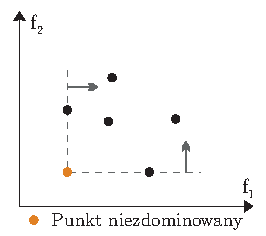
\includegraphics[]{/PSO/pareto/nondominated.pdf} \label{ss}}
	\subfloat[Front Pareto]{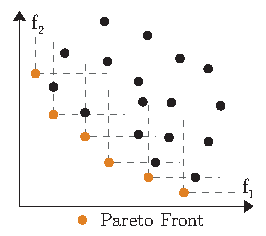
\includegraphics[]{/PSO/pareto/pareto_front.pdf} \label{ss}}
	\captionsetup{justification=centering}
	\caption{Wizualizacja definicji dominacji i Frontu Pareto}
	\label{ss}
\end{figure}








\subsection{Przykład teoretyczny}


